%\documentclass[12pt]{article}
%\usepackage[a4paper, margin=1in]{geometry} 
%\usepackage{graphicx} 
%\usepackage{hyperref}
%\usepackage{float}
%\usepackage{multicol}
%\usepackage{multirow}
%\usepackage[font=small, labelfont=bf]{caption}
%
%\begin{document}

%
% Confusion matrix 
%
\subsection{Confusion matrix}
The output of a model produces two false and two correct classifications. 

\begin{figure}[H]
  \centering
      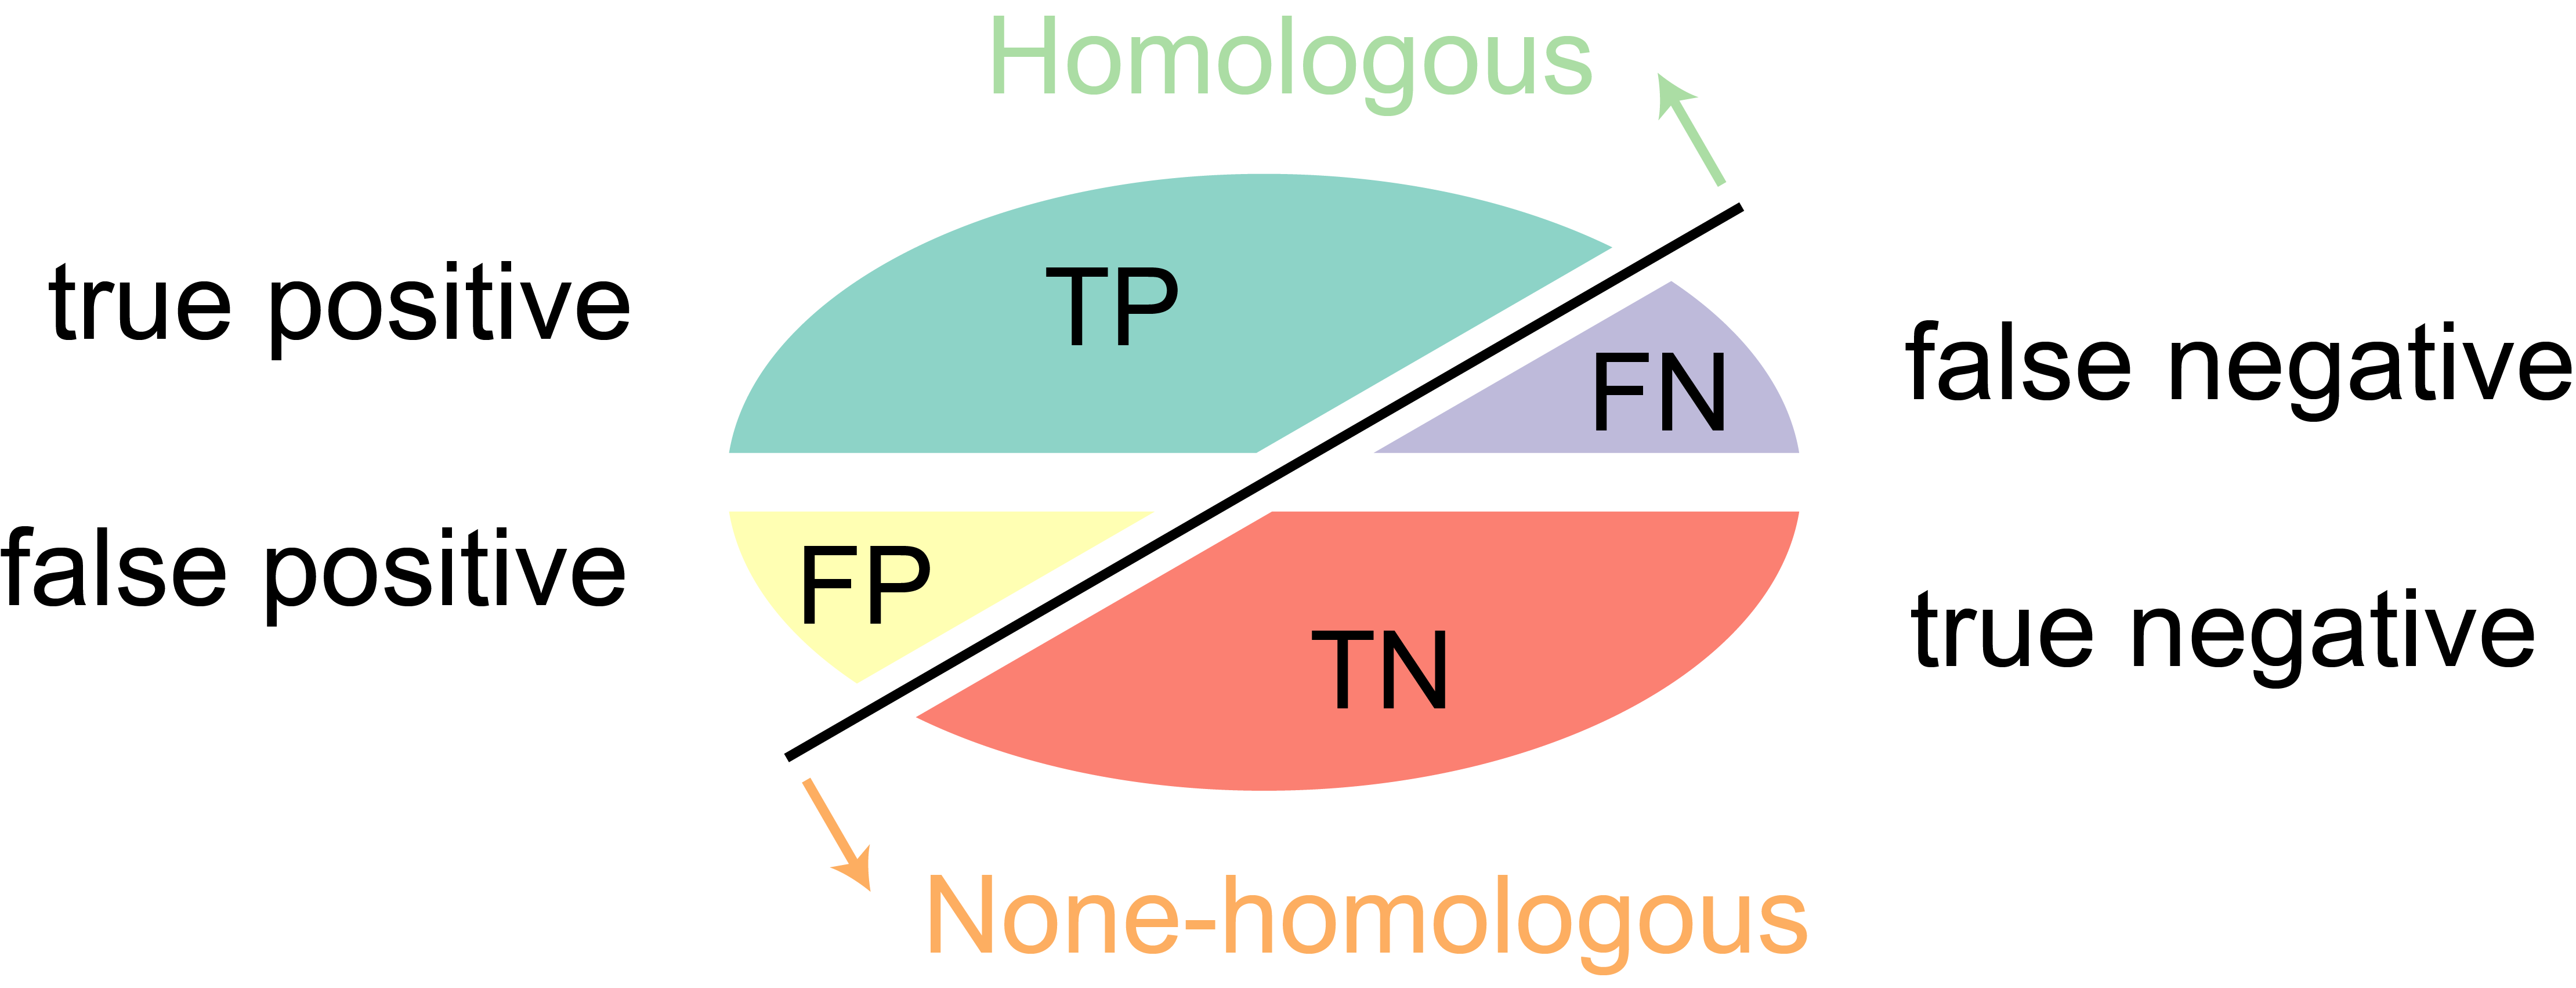
\includegraphics[width=0.4 \textwidth]{fig07/four_outcomes.png}
  \caption{Four outcomes of model classification}
\end{figure}


%
% Example of model output
%
\subsubsection*{Example of model output}
A test dataset contains 10 positives and 10 negative. 

\begin{figure}[H]
  \centering
      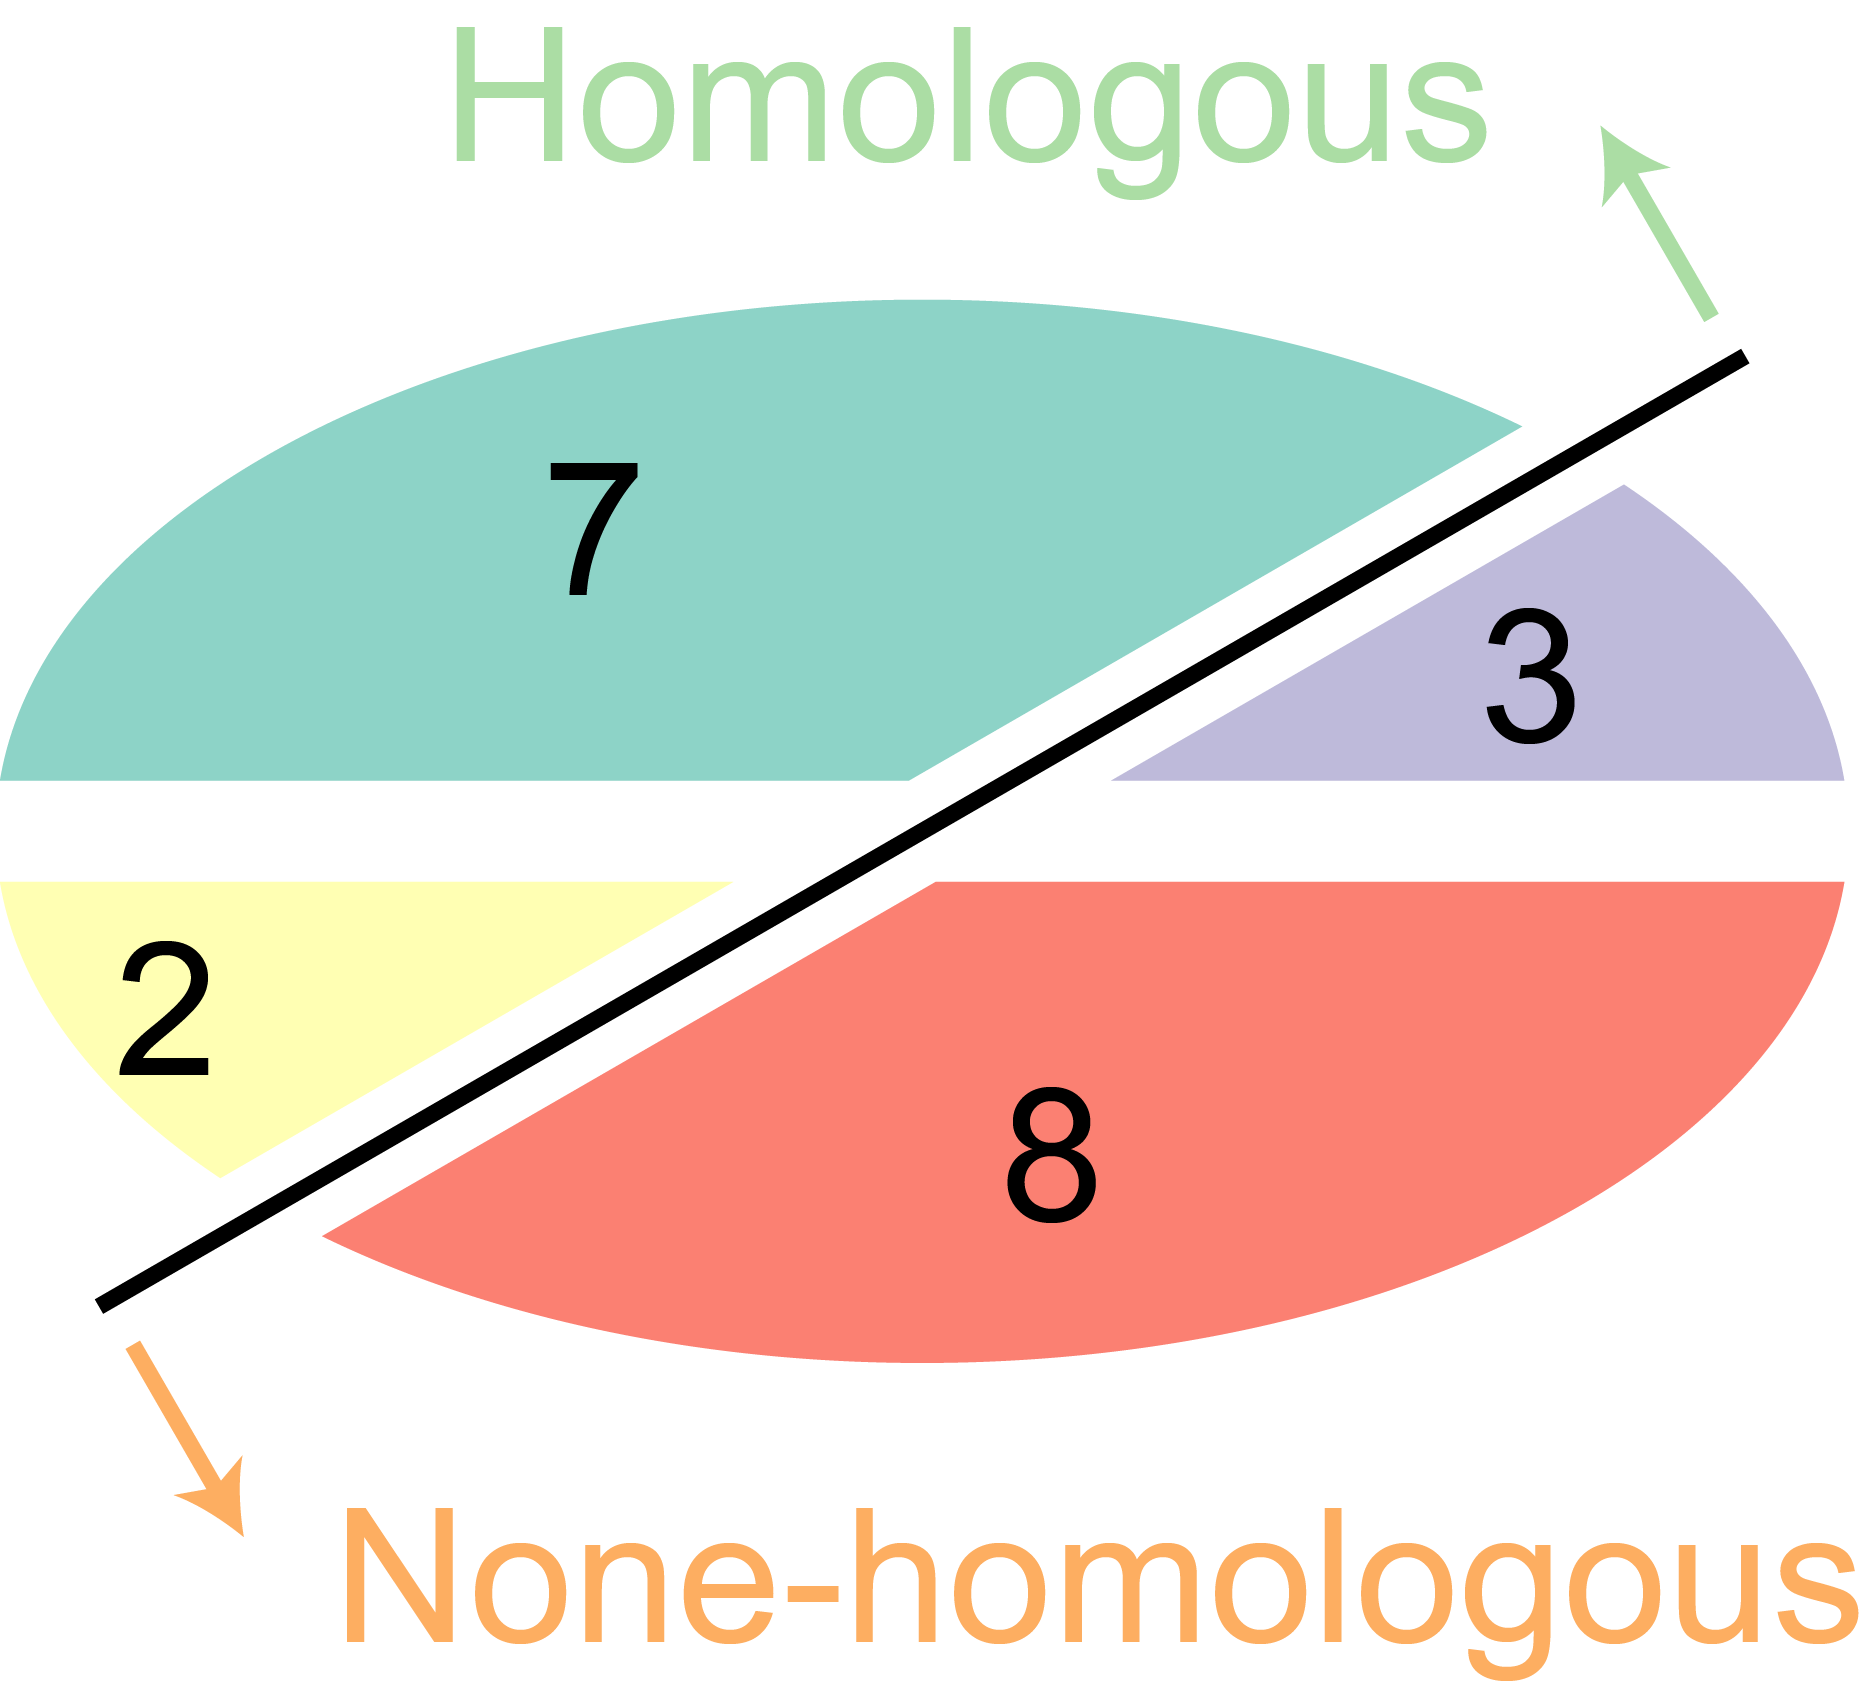
\includegraphics[width=0.2 \textwidth]{fig07/example_model_output.png}
  \caption{An example of the four outcomes}
\end{figure}

\begin{itemize}
\item 7 true positives
\item 8 true negatives
\item 2 false positives
\item 3 false negatives
\end{itemize}

%
% Confusion matrix
%
\subsubsection*{Confusion matrix}
The classification result can be formed into a matrix format.

\begin{table}[H]
\centering
\caption{Confusion matrix}
\begin{tabular}{ll|c|c|}
\cline{3-4}
                                                            &                & \multicolumn{2}{c|}{Test data}                                        \\ \cline{3-4} 
                                                            &                & \multicolumn{1}{l|}{Homologous} & \multicolumn{1}{l|}{Non-homologous} \\ \hline
\multicolumn{1}{|l|}{\multirow{2}{*}{Model classification}} & Homologous     & TP                              & FP                                  \\ \cline{2-4} 
\multicolumn{1}{|l|}{}                                      & Non-homologous & FN                              & TN                                  \\ \hline
\end{tabular}
\end{table}

%
% Example of confusion matrix
%
\subsubsection*{Example of confusion matrix}

\begin{table}[H]
\centering
\begin{tabular}{|l|l|}
\hline
7 TPs & 2 FPs \\ \hline
3 FNs & 8 TNs \\ \hline
\end{tabular}
\end{table}

\bigskip 

%\end{document}
